%=====================================================================
% MONTAGEM PREDIAL - PRATICA INTEGRADA DO PROJETO A ENTREGA
%=====================================================================

\section{Prática integrada — do projeto à execução}

\newcommand{\UnidadeDidaticaBase}{%
\draw[very thick](0,0)rectangle(8,6);
\draw[thick](0,2.4)--(8,2.4);
\draw[thick](5.0,2.4)--(5.0,6);
\draw[thick](2.8,0)--(2.8,2.4);
\draw[white,line width=5pt](1.0,0)--(2.0,0);\draw(1.0,0)--(2.0,1.0);
\draw[white,line width=5pt](1.0,2.4)--(1.9,2.4);\draw(1.0,2.4)--(1.9,3.3);
\draw[white,line width=5pt](5.5,2.4)--(6.4,2.4);\draw(5.5,2.4)--(6.4,3.3);
\draw[white,line width=5pt](2.8,.7)--(2.8,1.55);\draw(2.8,.7)--(3.65,1.55);
\node[font=\tiny\bfseries]at(2.5,5.5){SALA / QUARTO};
\node[font=\tiny\bfseries]at(6.5,5.5){COPA};
\node[font=\tiny\bfseries]at(1.4,1.95){BANHEIRO};
\node[font=\tiny\bfseries]at(5.4,1.2){ENTRADA / CIRCULAÇÃO};}

\begin{frame}{Desafio integrado — quatro competências no mesmo trabalho}
\centering
\begin{tikzpicture}[
  b/.style={draw=corPrim,fill=corDef!7,rounded corners,minimum width=2.25cm,minimum height=.78cm,align=center,font=\scriptsize},
  a/.style={-{Stealth},thick,corPrim}]
\node[b](l)at(-4.2,1){Ler e interpretar\\documentos};
\node[b](p)at(-1.4,-.7){Projetar\\e dimensionar};
\node[b](e)at(1.4,1){Executar\\e identificar};
\node[b](c)at(4.2,-.7){Ensaiar\\e entregar};
\draw[a](l)--(p)--(e)--(c);
\draw[a](c)to[bend left=30](l);
\end{tikzpicture}
\vspace{4mm}
\begin{caixaProjeto}[title=Regra da prática]
Toda alteração descoberta na execução volta ao projeto; todo circuito projetado termina em inspeção, ensaio e registro. Não existem notas separadas para desenho “bonito” e montagem que funciona por acaso.
\end{caixaProjeto}
\end{frame}

\begin{frame}{Unidade didática — arquitetura e programa}
\centering
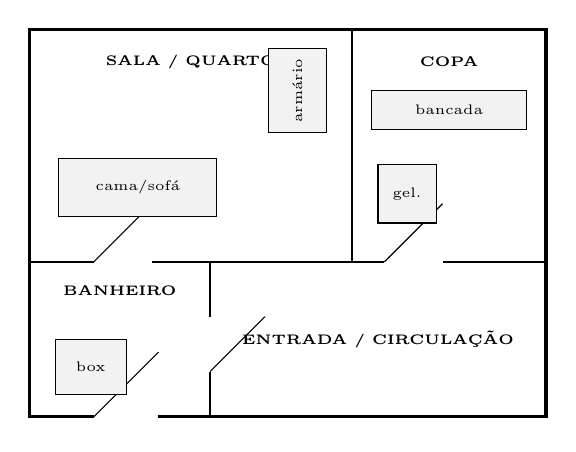
\begin{tikzpicture}[scale=.82,every node/.style={font=\scriptsize}]
\UnidadeDidaticaBase
\draw[fill=black!5](.45,3.1)rectangle(2.9,4.0);\node[font=\tiny]at(1.68,3.55){cama/sofá};
\draw[fill=black!5](3.7,4.4)rectangle(4.6,5.7);\node[font=\tiny,rotate=90]at(4.15,5.05){armário};
\draw[fill=black!5](5.3,4.45)rectangle(7.7,5.05);\node[font=\tiny]at(6.5,4.75){bancada};
\draw[fill=black!5](5.4,3.0)rectangle(6.3,3.9);\node[font=\tiny]at(5.85,3.45){gel.};
\draw[fill=black!5](.4,.35)rectangle(1.5,1.2);\node[font=\tiny]at(.95,.78){box};
\end{tikzpicture}
\vspace{1mm}
\begin{caixaObs}
Módulo de 48 m$^2$: iluminação com comando simples, paralelo e sensor; TUG gerais e de bancada; aquecedor 5,5 kW; ar-condicionado 1,2 kW; quadro próximo ao acesso.
\end{caixaObs}
\end{frame}

\begin{frame}{Planta elétrica — ler localização, circuito e comando}
\centering
\begin{tikzpicture}[scale=.92,every node/.style={font=\tiny}]
\UnidadeDidaticaBase
\SimQD{7.55}{1.25}{QD1}
\SimLuz{2.5}{4.4}\SimLuz{6.5}{4.4}\SimLuz{1.4}{1.2}\SimLuz{5.3}{1.2}
\SimInterruptor{1.1}{2.75}{S1p}\SimInterruptor{4.65}{2.75}{S2p}\SimInterruptor{5.4}{2.75}{S3}\SimInterruptor{2.45}{.45}{S4}
\foreach \x/\y in {.25/3.1,.25/5.4,4.75/3.1,4.75/5.4,5.25/5.8,7.75/5.8}{\SimTUG{\x}{\y}}
\foreach \x in {5.5,6.5,7.5}{\SimTUGM{\x}{5.1}}
\SimTUE{1.45}{.35}{AQ}\SimTUE{4.65}{5.65}{AC}
\draw[corAccent,dashed,thick](7.25,1.25)--(5.3,1.2)--(1.4,1.2)--(2.5,4.4)--(6.5,4.4);
\draw[corPrim,dashed,thick](7.25,1.0)--(7.2,3.1)--(4.75,3.1)--(.25,3.1);
\draw[corFix,dashed,thick](7.25,.75)--(1.45,.35);
\node[fill=white,corAccent,font=\tiny\bfseries]at(4.8,1.5){C1};
\node[fill=white,corPrim,font=\tiny\bfseries]at(6.8,3.4){C2/C3};
\node[fill=white,corFix,font=\tiny\bfseries]at(4,.6){C4};
\end{tikzpicture}
\vspace{1mm}
\scriptsize S1p/S2p: comando paralelo da sala; S3: copa; S4: banheiro; circulação por sensor no ponto L4. Rotas são didáticas e devem ser convertidas em comprimentos reais.
\end{frame}

\begin{frame}{Quadro de cargas — ponto de partida do trabalho}
\scriptsize
\begin{tabularx}{\textwidth}{c >{\bfseries}p{2.7cm}c c c c X}
\toprule
Circ. & Uso & Potência & $I_b$ em 220 V & DJ & Seção inicial & Comando/proteção \\
\midrule
C1 & iluminação & 0,40 kVA & 1,82 A & 10 A & 1,5 mm$^2$ & simples/paralelo/sensor \\
C2 & TUG sala/quarto & 1,20 kVA & 5,45 A & 16 A & 2,5 mm$^2$ & DR \\
C3 & TUG copa & 2,10 kVA & 9,55 A & 20 A & 2,5 mm$^2$ & DR \\
C4 & aquecedor & 5,50 kW & 25,0 A & 32 A 2P & 6 mm$^2$ & DR + dedicado \\
C5 & ar-condicionado & 1,20 kW & 5,93 A & 16 A & 2,5 mm$^2$ & dedicado \\
\bottomrule
\end{tabularx}
\begin{caixaAt}
Valores são hipóteses. Validar placa, método de instalação, temperatura, agrupamento, queda, curto, terminais, DR e especificações dos fabricantes antes de liberar a compra.
\end{caixaAt}
\end{frame}

\begin{frame}{Entrada didática — relacionar carga, padrão e QD}
\small
\begin{columns}[T,onlytextwidth]
\column{0.47\textwidth}
\[
P_{inst}=0{,}4+1{,}2+2{,}1+5{,}5+1{,}2=10{,}4\ \mathrm{kW}.
\]
Na tabela 220/380 V da NT.00001.EQTL Rev.09, uma unidade monofásica maranhense entre 8,1 e 12 kW usa, na referência didática:
\begin{itemize}
\item disjuntor do padrão: 63 A;
\item cobre do cliente: mínimo 10 mm$^2$;
\item demais colunas/notas obrigatórias.
\end{itemize}
\column{0.51\textwidth}
\begin{tikzpicture}[
  b/.style={draw=corPrim,fill=corDef!7,rounded corners,minimum width=2cm,minimum height=.68cm,align=center,font=\scriptsize}]
\node[b](r)at(0,3.6){rede / padrão};
\node[b](m)at(0,2.4){medição + DG};
\node[b](a)at(0,1.2){alimentador};
\node[b](q)at(0,0){QD1 + DPS + DR};
\node[b,draw=corNorma,fill=corNorma!7](pe)at(3,1.2){PE / BEP};
\draw[-{Stealth},thick,corPrim](r)--(m)--(a)--(q);
\draw[corNorma,thick](pe)--(q);\draw[corNorma,thick](pe.south)--(3,-.2)node[ground]{};
\end{tikzpicture}
\begin{caixaAt}
Dimensionar novamente o alimentador interno; não copiar automaticamente a seção do padrão.
\end{caixaAt}
\end{columns}
\end{frame}

\begin{frame}{Lista de condutores por trecho — exemplo de C1}
\scriptsize
\begin{tabularx}{\textwidth}{>{\bfseries}p{2.3cm}p{2.6cm}X X}
\toprule
Trecho & Formação funcional & Identificação & Observação \\
\midrule
QD1--CX1 & F + N + PE & C1-F, C1-N, C1-PE & alimentação da caixa principal \\
CX1--S1p & comum + V1 + V2 & C1-C, C1-V1, C1-V2 & primeiro paralelo \\
CX1--S2p & V1 + V2 + retorno & C1-V1, C1-V2, C1-R1 & segundo paralelo \\
CX1--L1 & retorno + N + PE & C1-R1, C1-N, C1-PE & luminária da sala \\
CX1--S3--L2 & F + retorno / R + N + PE & C1-F/R2/N/PE & copa \\
CX1--sensor--L4 & F + N + saída / R + N + PE & C1-F/N/R4/PE & conferir modelo do sensor \\
\bottomrule
\end{tabularx}
\begin{caixaProjeto}[title=Atividade]
Marcar esses códigos na planta, na lista de cabos, nas anilhas e na folha de continuidade. Qualquer alteração deve aparecer nos quatro lugares.
\end{caixaProjeto}
\end{frame}

\begin{frame}{Unifilar simplificado do QD1}
\centering
\begin{tikzpicture}[
  b/.style={draw=corPrim,fill=corDef!7,rounded corners,minimum width=1.75cm,minimum height=.62cm,align=center,font=\tiny}]
\node[b](dg)at(0,4.0){DG 2P 63 A};
\node[b](dps)at(0,3.0){DPS + barras N/PE};
\node[b,draw=corNorma,fill=corNorma!7](dr)at(0,2.0){DR/RCBO conforme projeto};
\node[b](c1)at(-4.8,.3){C1 luz\\10 A / 1,5};
\node[b](c2)at(-2.4,-.7){C2 TUG\\16 A / 2,5};
\node[b](c3)at(0,.3){C3 copa\\20 A / 2,5};
\node[b](c4)at(2.4,-.7){C4 AQ\\32 A / 6};
\node[b](c5)at(4.8,.3){C5 AC\\16 A / 2,5};
\draw[-{Stealth},thick,corPrim](dg)--(dps)--(dr);
\foreach \x in {c1,c2,c3,c4,c5}{\draw[-{Stealth},thick,corPrim](dr)--(\x);}
\end{tikzpicture}
\begin{caixaObs}
O aluno deve completar: capacidade de interrupção, tipo/polos do DR, ligação do DPS, método/seções finais, correntes corrigidas, quedas, comprimentos e bornes.
\end{caixaObs}
\end{frame}

\begin{frame}{Lista de materiais — comprar por função e requisito}
\scriptsize
\begin{tabularx}{\textwidth}{c >{\bfseries}p{3.0cm}c X}
\toprule
Item & Descrição & Quant. & Informação para seleção \\
\midrule
01 & quadro de distribuição & 1 & módulos, reserva, barras, IP e corrente \\
02 & disjuntores/DPS/DR & conjunto & dados completos do unifilar \\
03 & cabos 1,5/2,5/6/10 mm$^2$ & por medição & classe, isolação, cor e comprimento + reserva \\
04 & eletrodutos e caixas & por rota & diâmetro, ocupação, curvas, fixação e acesso \\
05 & tomadas, interruptores e sensor & por planta & corrente, tensão, módulos, IP e compatibilidade LED \\
06 & luminárias e driver & 4 conjuntos & fluxo, potência, CCT, IRC e montagem \\
07 & terminais/conectores & por borne & seção, classe, corrente e ferramenta \\
08 & etiquetas/anilhas & conjunto & códigos do projeto e resistência ambiental \\
\bottomrule
\end{tabularx}
\begin{caixaAt}
Comprimento de cabo vem da rota executiva, não da distância em linha reta da planta. Incluir subidas, descidas, curvas, quadro, caixas e folgas previstas — sem sobras ocultas excessivas.
\end{caixaAt}
\end{frame}

\begin{frame}{Plano de execução — sequência e pontos de espera}
\scriptsize
\begin{enumerate}
\item revisar documentos, compatibilizar e liberar marcação;
\item marcar caixas, quadro, eixos e cotas;
\item instalar infraestrutura e conferir rotas;
\item \textbf{ponto de espera 1}: inspeção antes de fechar paredes/forro;
\item limpar/provar eletrodutos e lançar cabos identificados;
\item terminar caixas, cargas e QD com torque controlado;
\item \textbf{ponto de espera 2}: inspeção e ensaios desenergizados;
\item corrigir não conformidades e atualizar desenhos;
\item energizar circuito a circuito e testar funções;
\item \textbf{ponto de espera 3}: aceite, as built e entrega.
\end{enumerate}
\begin{caixaObs}
Cada equipe recebe uma frente, mas a passagem de serviço depende do registro da anterior. Isso ensina execução como processo coordenado, não como tarefas soltas.
\end{caixaObs}
\end{frame}

\begin{frame}{Ordem de serviço — exemplo para C1}
\scriptsize
\begin{tabularx}{\textwidth}{>{\bfseries}p{2.4cm}X X}
\toprule
Campo & Conteúdo & Evidência \\
\midrule
Escopo & montar C1: sala paralela, copa simples, banheiro e sensor & planta PE-01 + diagrama DE-01 R00 \\
Fontes & QD1 e qualquer retorno/temporário & lista de bloqueio e ausência de tensão \\
Materiais & cabos, mecanismos, caixas, terminais e luminárias & lote e conferência de recebimento \\
Ferramentas & decapador, crimpador, torquímetro, instrumentos & inspeção e calibração aplicável \\
Conexões & conforme lista de bornes e fios & inspeção ponto a ponto \\
Ensaios & PE, isolação, polaridade e função & folha E-C1 \\
Critério & projeto, procedimento e fabricante & aceite/NC/retrabalho \\
\bottomrule
\end{tabularx}
\begin{caixaAt}
A ordem de serviço não autoriza improvisar alteração. Divergência de campo gera consulta, decisão registrada e revisão correspondente.
\end{caixaAt}
\end{frame}

\begin{frame}{Cartões de falha — aprender diagnóstico sem adivinhação}
\small
\begin{columns}[T,onlytextwidth]
\column{0.49\textwidth}
\begin{caixaFix}[title=Falhas possíveis]
\begin{itemize}
\item comum do paralelo trocado com V1;
\item neutro de C2 na barra do DR errado;
\item PE interrompido em uma tomada;
\item sensor com L e L$'$ invertidos;
\item terminal subcrimpado;
\item etiqueta C4 aplicada no cabo C5;
\item borne do QD sem torque;
\item alteração de rota não documentada.
\end{itemize}
\end{caixaFix}
\column{0.49\textwidth}
\begin{caixaProjeto}[title=Método obrigatório]
\begin{enumerate}
\item definir sintoma;
\item tornar seguro;
\item ler documentos;
\item formular hipótese;
\item escolher ensaio discriminante;
\item corrigir a causa;
\item reensaiar proteção e função;
\item registrar e atualizar as built.
\end{enumerate}
\end{caixaProjeto}
\end{columns}
\end{frame}

\begin{frame}{Ficha de inspeção — aceitar ou rejeitar com evidência}
\scriptsize
\begin{tabularx}{\textwidth}{c X c c X}
\toprule
ID & Verificação & C & NC & Observação/evidência \\
\midrule
I-01 & caixas e cotas correspondem à planta & $\square$ & $\square$ & \\
I-02 & rotas, diâmetros e segregação conferidos & $\square$ & $\square$ & \\
I-03 & cabos, seções e identificações conferem & $\square$ & $\square$ & \\
I-04 & terminais e torques registrados & $\square$ & $\square$ & \\
I-05 & neutros separados por DR e PE contínuo & $\square$ & $\square$ & \\
I-06 & barreiras, tampas e acesso recompostos & $\square$ & $\square$ & \\
I-07 & planta, quadro e unifilar coerentes & $\square$ & $\square$ & \\
I-08 & ensaios anexos atendem aos critérios & $\square$ & $\square$ & \\
\bottomrule
\end{tabularx}
\begin{caixaObs}
“C” exige evidência; campo vazio não significa conforme. “NC” precisa de responsável, prazo, correção e revalidação.
\end{caixaObs}
\end{frame}

\begin{frame}{Dossiê final da unidade didática}
\scriptsize
Cada grupo entrega:
\begin{enumerate}
\item briefing e levantamento da arquitetura;
\item planta elétrica cotada, legenda e detalhes;
\item memória de cargas e dimensionamentos;
\item quadro de cargas e unifilar;
\item esquemas funcional, multifilar e de ligação;
\item lista de cabos, bornes e materiais;
\item análise de risco, ordem de serviço e checklists;
\item registros de torque, inspeção e ensaios;
\item relatório de falha/correção e reensaio;
\item as built e apresentação da instalação funcionando.
\end{enumerate}
\begin{caixaProjeto}[title=Defesa oral]
O avaliador aponta qualquer componente. O aluno deve mostrar onde ele aparece na planta, no quadro, no esquema, na lista de materiais e no relatório de ensaio.
\end{caixaProjeto}
\end{frame}

\begin{frame}{Rubrica — o aluno realmente aprendeu?}
\scriptsize
\begin{tabularx}{\textwidth}{>{\bfseries}p{3.6cm}c X}
\toprule
Competência & Peso & Evidência de domínio \\
\midrule
Leitura/interpretação & 25\% & segue circuitos, referências e bornes sem depender de memorização \\
Projeto/dimensionamento & 25\% & premissas, cálculos e documentos são coerentes e verificáveis \\
Ligação/montagem & 25\% & executa com identificação, ferramenta, terminal, torque e acabamento corretos \\
Segurança/ensaios & 20\% & controla energia, escolhe método, mede, interpreta e registra \\
Comunicação/as built & 5\% & outro profissional entende e mantém a instalação entregue \\
\bottomrule
\end{tabularx}
\begin{caixaAt}
Falha crítica de segurança reprova a prática independentemente da soma. Instalação energizada e funcional não compensa ausência de PE, barreira, proteção ou procedimento.
\end{caixaAt}
\end{frame}

\begin{frame}{Resultado esperado da formação predial}
\centering
\begin{tikzpicture}[
  b/.style={draw=corPrim,fill=corDef!7,rounded corners,minimum width=2.35cm,minimum height=.82cm,align=center,font=\scriptsize},
  a/.style={-{Stealth},very thick,corPrim}]
\node[b](l)at(-4.5,0){Lê\\planta, tabela e diagrama};
\node[b](p)at(-1.5,0){Projeta\\calcula e documenta};
\node[b](e)at(1.5,0){Executa\\liga e identifica};
\node[b](v)at(4.5,0){Verifica\\mede e entrega};
\draw[a](l)--(p)--(e)--(v);
\end{tikzpicture}
\vspace{6mm}
\begin{caixaProjeto}[title=Competência profissional integrada]
O aluno não apenas reproduz um desenho: entende a intenção, confere os dados, transforma o projeto em instalação, prova o resultado e mantém a documentação fiel ao que foi construído.
\end{caixaProjeto}
\end{frame}
